 \iffalse
\let\negmedspace\undefined
\let\negthickspace\undefined
\documentclass[a4,12pt,onecolumn]{IEEEtran}
\usepackage{amsmath,amssymb,amsfonts,amsthm}
\usepackage{algorithmic}
\usepackage{graphicx}
\usepackage{textcomp}
\usepackage{xcolor}
\usepackage{txfonts}
\usepackage{listings}
\usepackage{enumitem}
\usepackage{mathtools}
\usepackage{gensymb}
\usepackage[breaklinks=true]{hyperref}
\usepackage{tkz-euclide}
\usepackage{listings}
\usepackage{gvv}
\begin{document}
\title{
\Huge\textbf{Discrete Assignment}\\
\Huge\textbf{EE1205} Signals and Systems\\
}
\large\author{Kurre Vinay\\EE23BTECH11036}
\maketitle
\textbf{Question 11.9.3.8:}
Find the sum to indicated number of term in each of the geometric progressions in $\sqrt{7} ,\sqrt{21} , 3\sqrt{7}, ....n$ terms\\
\solution
\fi
\begin{table}[h!]
 \begin{center}
\begin{tabular}{|c|c|c|}
   \hline
   variable&value&description  \\
   \hline
   $x(0)$ & $ \sqrt{7} $& first term of the geometric progession\\
   \hline
   $r$ & $\sqrt{3}$ & common ratio of the geometeric progression\\
   \hline
   $x(n)$ & $\sqrt{7(3^{n})}u\brak{n}$& $n^{th}$ term of the geometric progession\\
   \hline
   $y(n)$ &$\frac{x(0)(r^{n+1}-1)}{r-1}u\brak{n}$ &Sum of the n term of the geometric progression\\
   \hline 
\end{tabular}
\caption{Input parameters}
\end{center}
\end{table}

\begin{align}
X\brak{z} &= x\brak{0}\brak{\frac{1}{1-rz^{-1}}}, \quad{|rz^{-1}|<1}\\
y\brak{n} &= x\brak{n}*u\brak{n}\\
Y\brak{z} &= X\brak{z}U\brak{z}\\
&=\sqrt{7}\brak{\frac{1}{1-\sqrt{3}z^{-1}}}\brak{\frac{1}{1-z^{-1}}} ,\quad{|z|>\sqrt{3}}\\
&=\brak{\frac{\sqrt{7}}{\sqrt{3}-1}}\brak{\brak{\frac{\sqrt{3}}{1-\sqrt{3}z^{-1}}}-\brak{\frac{1}{1-z^{-1}}}}\\
\frac{1}{1-rz^{-1}} &\xleftrightarrow{\mathcal{Z}^{-1}}  r^nu(n), \quad{|z|>r}\\
y\brak{n} &= \sqrt{7}\brak{\frac{\sqrt{3}^{n+1}-1}{\sqrt{3}-1}}u(n) , \quad{|z|>\sqrt{3}}
\end{align}

\begin{figure}[ht!]
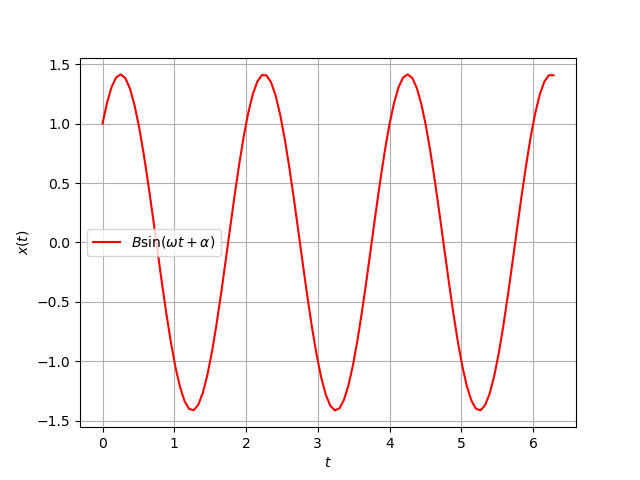
\includegraphics[width=\columnwidth]{figs/fig2.png}
\caption{\large{STEM PLOT OF $y\brak{n}$}}
\end{figure}
